% !TEX root=ricardo_draft.tex
% In this section we evaluate our framework for modeling fairness.
We test our approach on two practical problems that require fairness, the first is \emph{prediction of success in law school} and the second is \emph{separating actual and perceived criminality in police stops}. For each problem we construct causal models, and make explicit how unfairness may affect observed and unobserved variables in the world. Given these models we derive counterfactually fair predictors, and predict latent variables such as a person's `criminality' (which may be useful for predicting crime) as well as their `perceived criminality' (which may be due to prejudices based on race and sex). We analyze empirically how counterfactually fair the unaware and full predictors are, assuming knowledge of the correct causal model, and compare the prediction accuracies of all models. Finally we judge how well our counterfactually fair `criminality' score satisfies demographic parity.
% We analyze how realistic our models are by comparing our observations with data generated from the model. 



\subsection{Law school success}
\label{sec:law-school-success}
% From 1991 to 1996
The Law School Admission Council
conducted a survey across 163 law
schools in the United States \cite{wightman1998lsac}. % The survey was
% designed to assess `the law school experience of minority students, as
% well as their ultimate entry into the profession'.
It contains information on 21,790 law students such as their entrance exam scores (LSAT), their grade-point
average (GPA) collected prior to law school, and their first year average grade
(FYA). %, and following Law
%School i.e. whether students passed the final examination, the `bar
%exam' (P)).

Given this data, a school may wish to predict if an applicant will
have a high FYA. % from information about their academic performance
% before law school.
The school would also like to make sure these
predictions are not biased by an individual's race and sex. However,
the LSAT, GPA, and FYA scores, may be biased due to social factors. % Our approach will use variables that are
% counterfactually fair for prediction.
We compare our framework with
two unfair baselines: 1. \textbf{Full}: the standard technique of
using all features, including sensitive features such as race and sex
to make predictions; 2. \textbf{Unaware}: fairness through
unawareness, where we do not use race and sex as features. For comparison, we generate predictors $\hat Y$ for all models using logistic regression.


\paragraph{Fair prediction.}
As described in Section~\ref{sec:limit-guide-model}, there are three ways in which we can model a counterfactually fair predictor of FYA. Level 1 uses any features which are not descendants of race and sex for prediction. Level 2 models latent `fair' variables which are parents of observed variables. These variables are independent of both race and sex. Level 3 models the data using an additive error model, and uses the independent error terms to make predictions. These models make increasingly strong assumptions corresponding to increased predictive power. We split the dataset 80/20 into a train/test set, preserving label balance, to evaluate the models.

As we believe LSAT, GPA, and FYA are all biased by race and sex, we
cannot use any observed features to construct a counterfactually fair
predictor as described in Level 1. % Instead we would need to resort to a
% constant predictor% , such as the mean of FYA over the training set
% . % As this model is trivial we do not consider it. 

In Level 2, we postulate that a latent variable: a student's \textbf{knowledge} (K), affects GPA, LSAT, and FYA scores. The causal graph corresponding to this model is shown in Figure~\ref{figure.law_school}, (\textbf{Level 2}). This is a short-hand for the distributions:
\begin{align}
\mbox{GPA} &\sim {\cal N}(b_{G} + w_{G}^K K + w_{G}^R R + w_{G}^S S, \sigma_{G}) \nonumber \\
\mbox{LSAT} &\sim \textrm{Poisson}(\exp(b_{L} + w_{L}^K K + w_{L}^R R + w_{L}^S S)) \nonumber \\
\mbox{FYA} &\sim {\cal N}(w_{F}^K K + w_{F}^R R + w_{F}^S S, 1) \nonumber \\
K &\sim {\cal N}(0,1) \nonumber
\end{align}
% As FYA is already standardized to have mean $0$ and standard deviation $1$ we do not learn bias and standard deviation terms.
We perform inference on this model using an observed training set to estimate the posterior distribution of $K$. We use the probabilistic programming language Stan \cite{rstan} to learn $K$. We call the predictor constructed using $K$, \textbf{Fair $K$}.


\begin{figure}[th]
\begin{center}
\vspace{-1ex}
\centerline{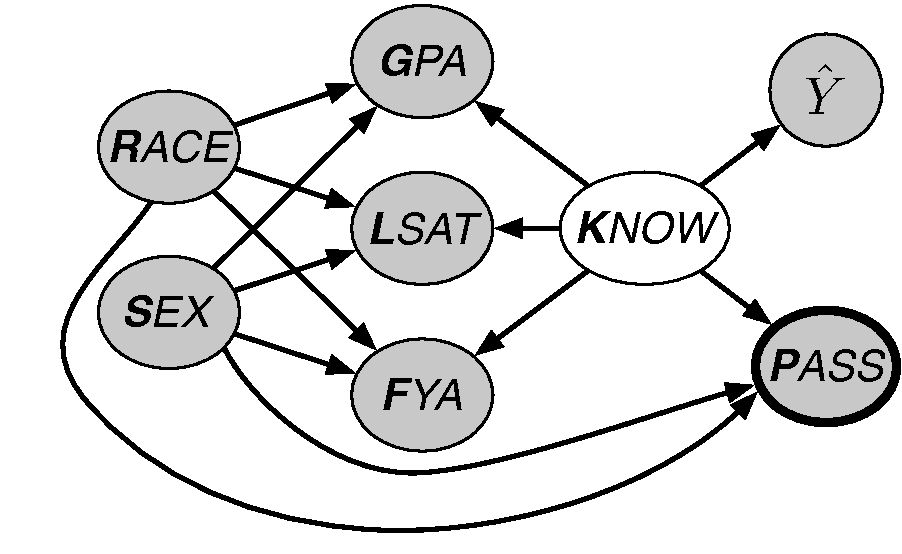
\includegraphics[width=0.8\columnwidth]{law_school_model}}
\vspace{-2ex}
\caption{A causal model for the problem of predicting law school success fairly.\label{figure.law_school}\vspace{-2ex}}
\vspace{-2ex}
\end{center}
\end{figure}

\begin{table}
\centering
\caption{Prediction results using logistic regression. Note that we must sacrifice a small amount of accuracy to ensuring counterfactually fair prediction (Fair $K$, Fair Add), versus the models that use unfair features: GPA, LSAT, race, sex (Full, Unaware).}\label{table.pred_law}
\begin{tabular}{ccccc} 
\hline
 &  {\bf Full} & {\bf Unaware} & {\bf Fair $K$} & {\bf Fair Add} \\
\hline
RMSE & 0.873 & 0.894 & 0.929 & 0.918 \\
%\bf{Method} & %\multicolumn{2}{c}{\bf Full} & \multicolumn{2}{c}{\bf Unaware} & \multicolumn{2}{c}{\bf Fair L2} & \multicolumn{2}{c}{\bf Fair L3} \\
\hline
\end{tabular}
\end{table}

\begin{figure}[th]
\begin{center}
 \label{figure.counterfactual}
\vspace{-1ex}
\centerline{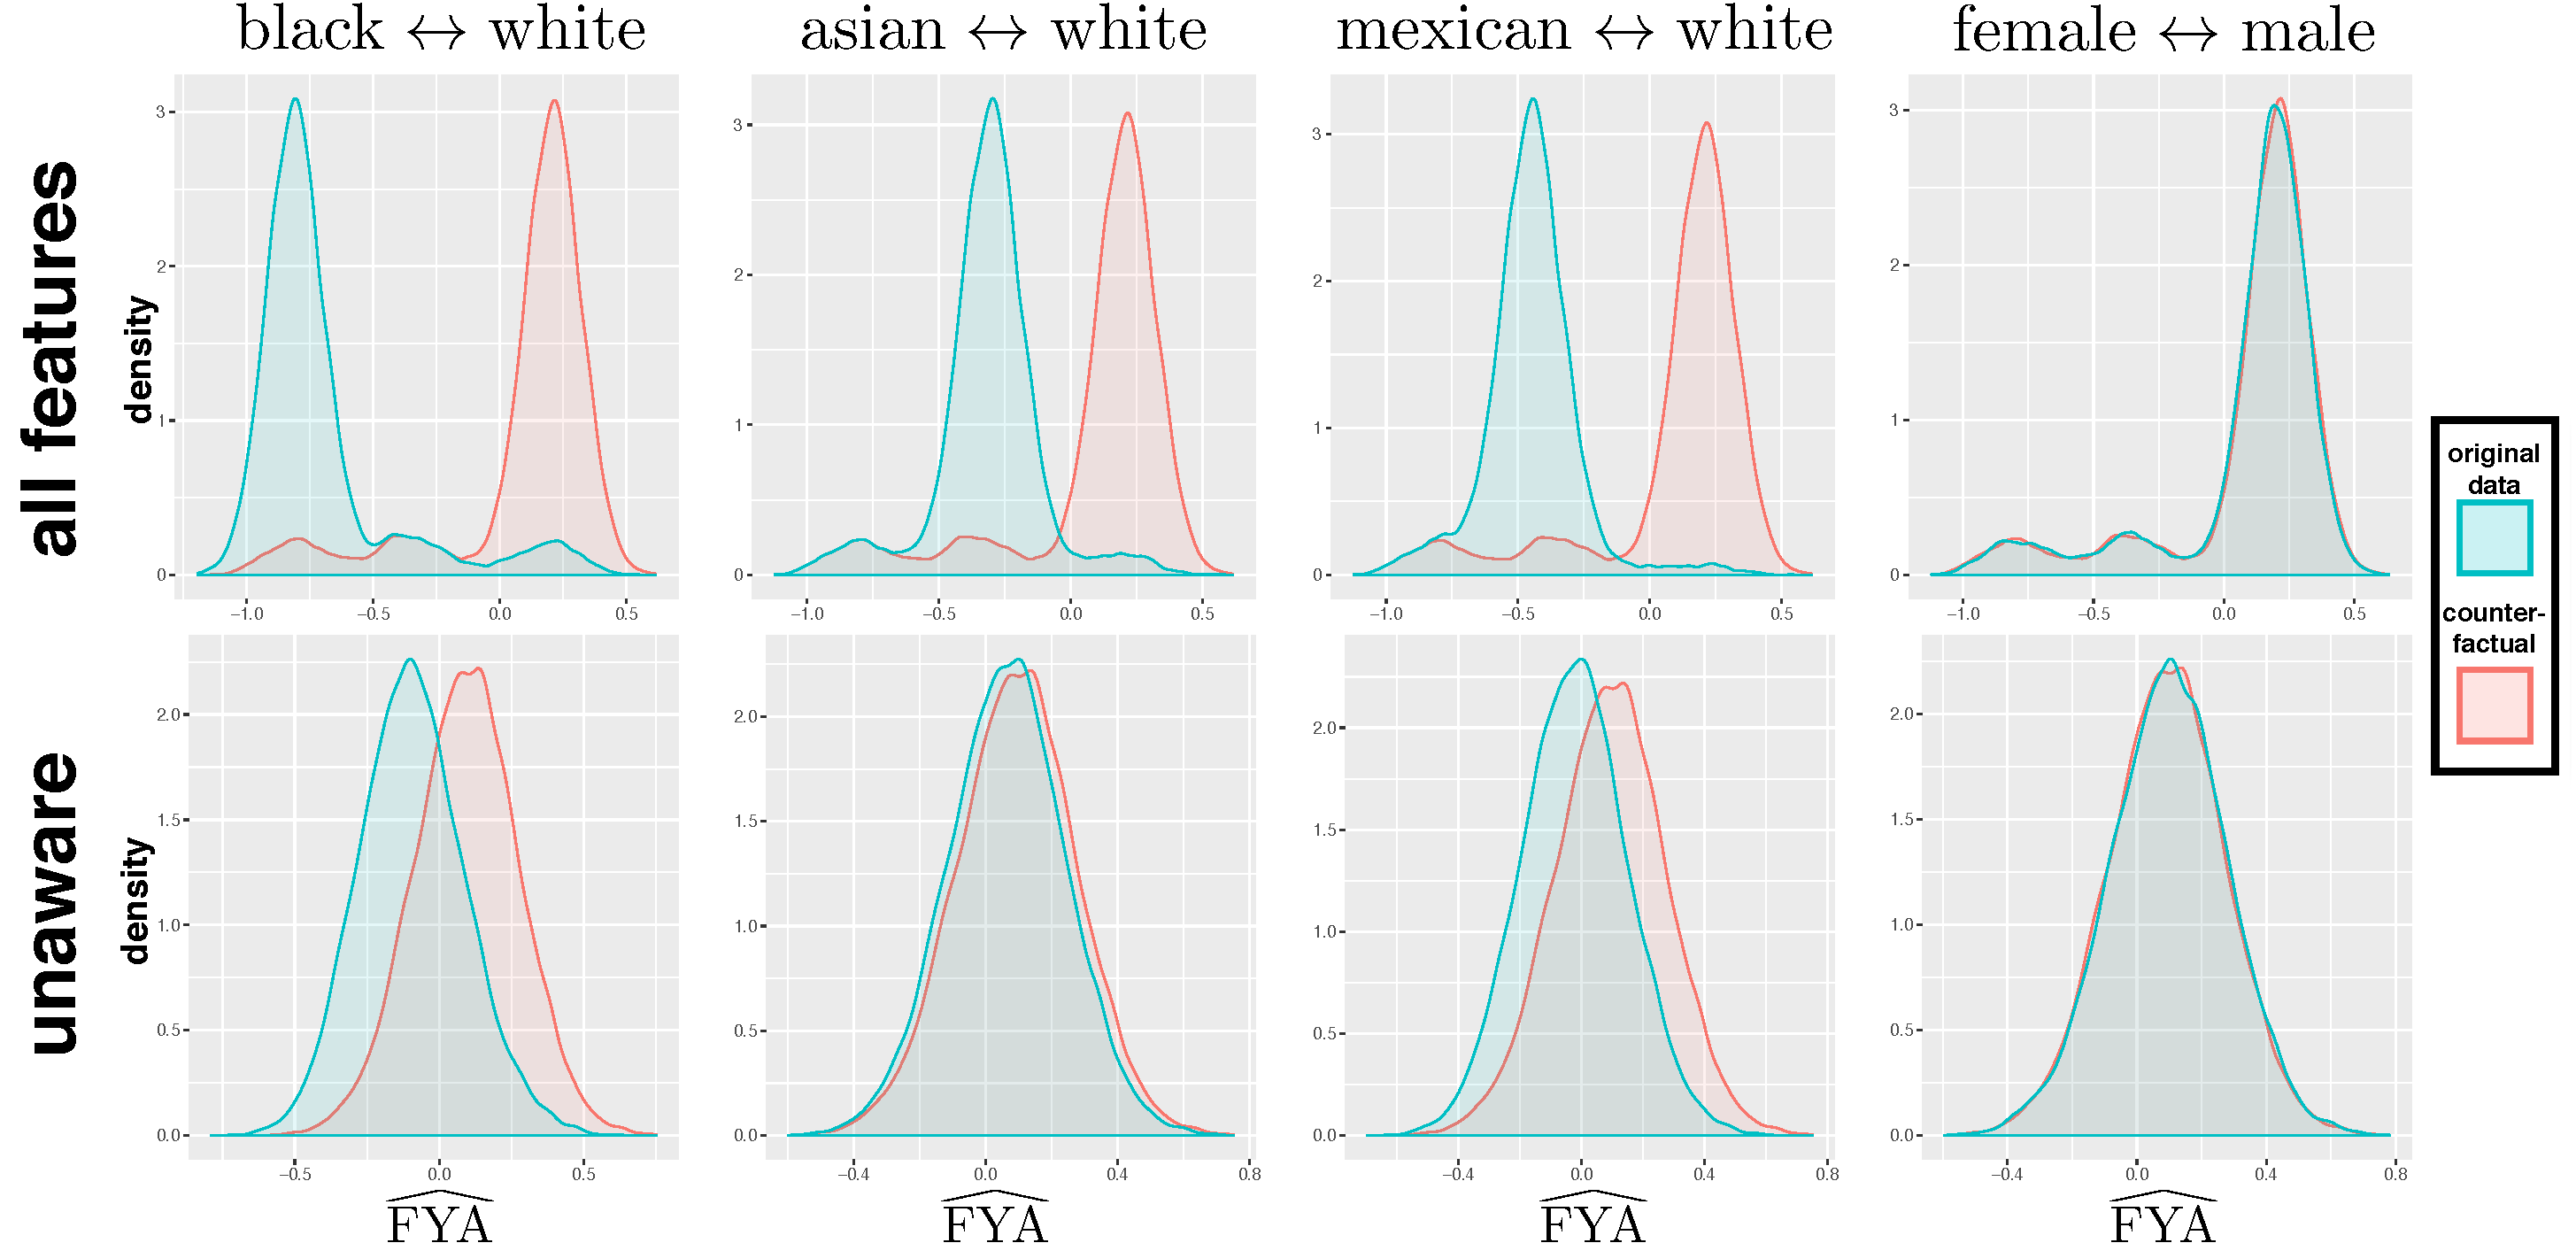
\includegraphics[width=\columnwidth]{counterfactual}}
\vspace{-2ex}
\caption{Density plots of predicted $\mbox{FYA}_a$ and $\mbox{FYA}_{a'}$.}
\vspace{-2ex}
\end{center}
\end{figure}

In Level 3, we model GPA, LSAT, and FYA as continuous variables with additive error terms independent of race and sex (that may in turn be correlated with one-another). This model is shown in Figure~\ref{figure.law_school}, (\textbf{Level 3}), and is expressed by: % the equations:
\begin{align}
\mbox{GPA} &= b_{G} + w_{G}^R R + w_{G}^S S + \epsilon_G, \;\; \epsilon_G \sim p(\epsilon_G) \nonumber \\
\mbox{LSAT} &= b_{L} + w_{L}^R R + w_{L}^S S + \epsilon_L, \;\; \epsilon_L \sim p(\epsilon_L) \nonumber \\
\mbox{FYA} &= b_{F} + w_{F}^R R + w_{F}^S S + \epsilon_F, \;\; \epsilon_F \sim p(\epsilon_F) \nonumber
\end{align}
We estimate the error terms $\epsilon_G,\epsilon_L$ by first fitting two models that each use race and sex to individually predict GPA and LSAT. We then compute the residuals of each model (e.g., $\epsilon_G \!=\! \mbox{GPA} \!-\! \hat{Y}_{\scriptsize\mbox{GPA}}(R,S)$). We use these residual estimates of $\epsilon_G,\epsilon_L$ to predict FYA. We call this \emph{Fair Add}.


% impacts these features.

% We propose to model the law school data as shown in
% Figure~\ref{figure.law_school}. We suspect that variables race and sex
% affect student performance (e.g. GPA, LSAT, and FYA) due to factors
% such as cultural norms, which assume that individuals of a certain
% race or sex are `better suited' to be lawyers. Such beliefs could
% adversely impact students who do not fit these norms. Instead we would
% like to model the latent \emph{knowledge} (K) of a student, which also
% impacts these features. 
% We can then construct a predictor that
% predicts FYA fairly using knowledge. It is easy to show that such a predictor
% is counterfactually fair, whereas a predictor that uses features GPA and
% LSAT is not (in this case even including race and sex as
% features cannot correct this, as can be done in the linear case). The
% causal 
 %; %3. \textbf{Variational Fair Autoencoder (VFAE)} \cite{louizos2015variational}, a recent approach that works to learn a fair representation of the original data.
% compute counterfactuals for both race and sex

\begin{figure*}[!th]
\begin{center}
\vspace{-2ex}
\centerline{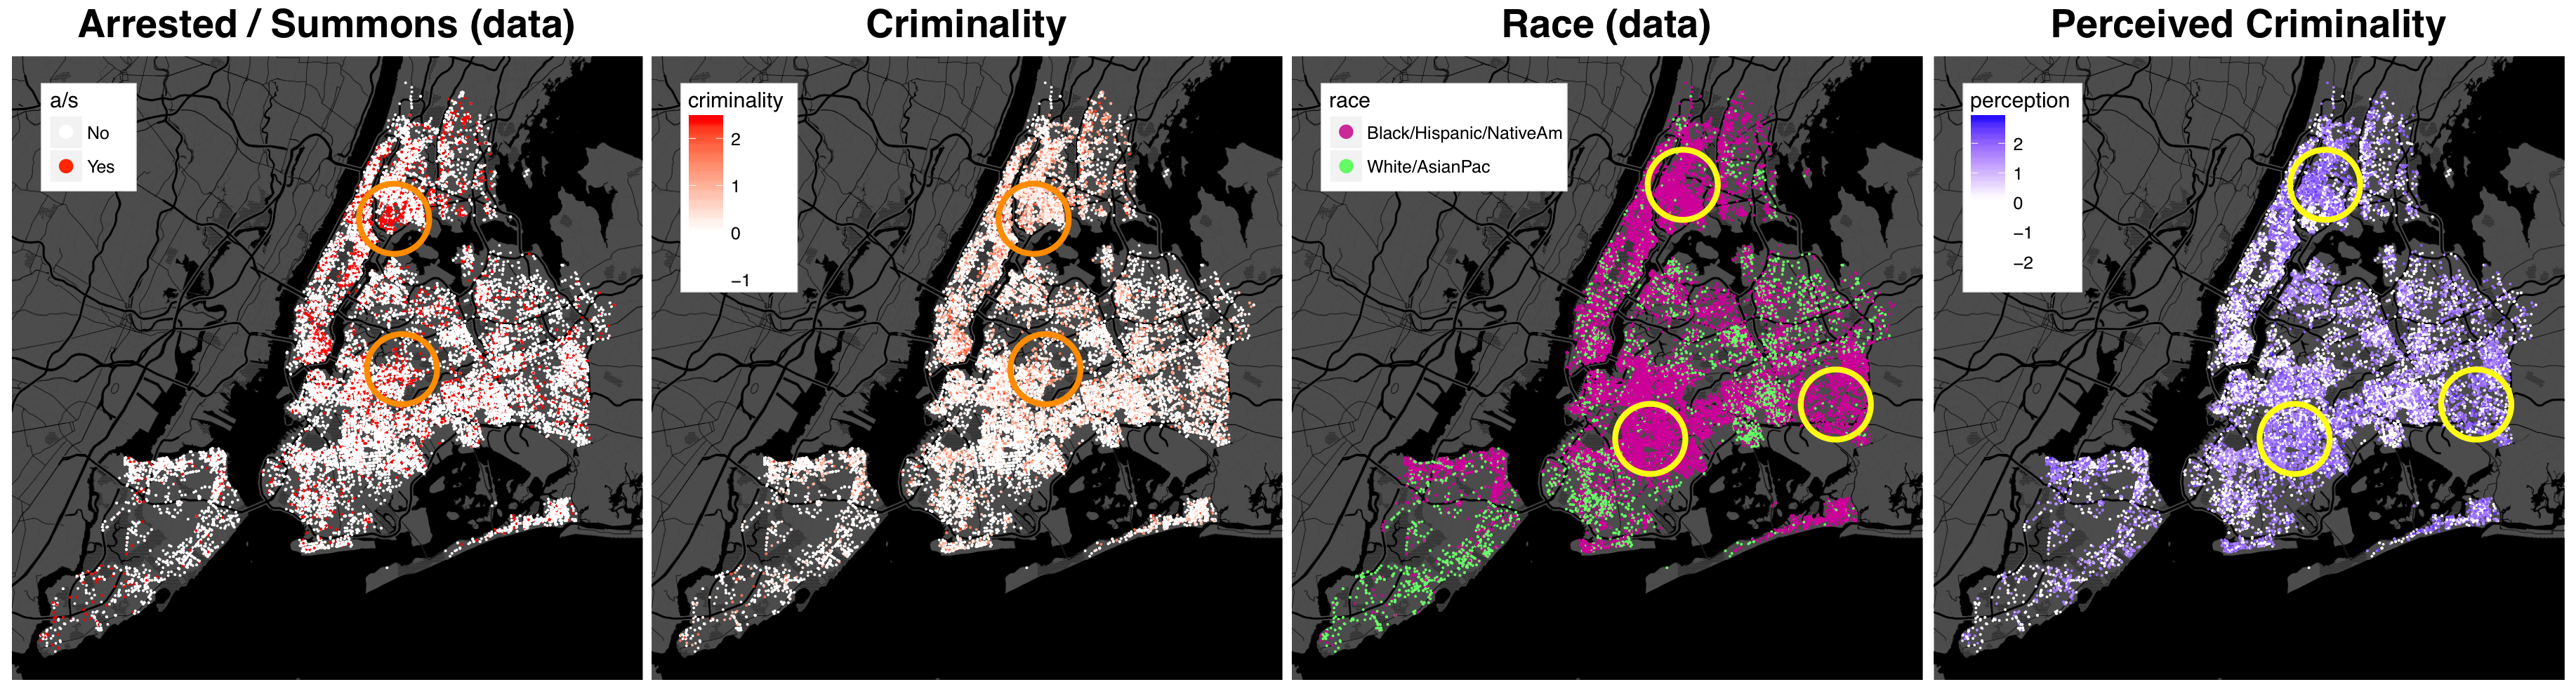
\includegraphics[width=\textwidth]{stop_and_frisk_graphs.png}}
\vspace{-2ex}
\caption{Understanding criminality. The above maps show the decomposition of stop and search data in New York into factors based on perceived criminality (a race dependent variable) and latent criminality (a race neutral measure). See section~\ref{sec:true-vs.-perceived}.     \label{figure.criminality}\vspace{-7ex}}
\end{center}
%\vspace{-3ex}
\end{figure*}

\paragraph{Accuracy.}
We compare the RMSE achieved by logistic regression for each of the models on the test set in Table~\ref{table.pred_law}.  The \textbf{Full} model achieves the lowest RMSE as it uses race and sex to more accurately reconstruct FYA. Note that in this case, this model is not fair even if the data was generated by one of the models shown in Figure~\ref{figure.law_school} as it corresponds to Scenario 3. The (also unfair) \textbf{Unaware} model still uses the unfair variables GPA and LSAT, but because it does not use race and sex it cannot match the RMSE of the \textbf{Full} model. As our models satisfy counterfactual fairness, they trade off some accuracy. Our first model \textbf{Fair $K$} uses weaker assumptions and thus the RMSE is highest. Using the Level 3 assumptions, as in \textbf{Fair Add} we produce a counterfactually fair model that trades lower RMSE for slightly weaker assumptions.

\begin{figure}[th]
\begin{center}
\vspace{-1ex}
\centerline{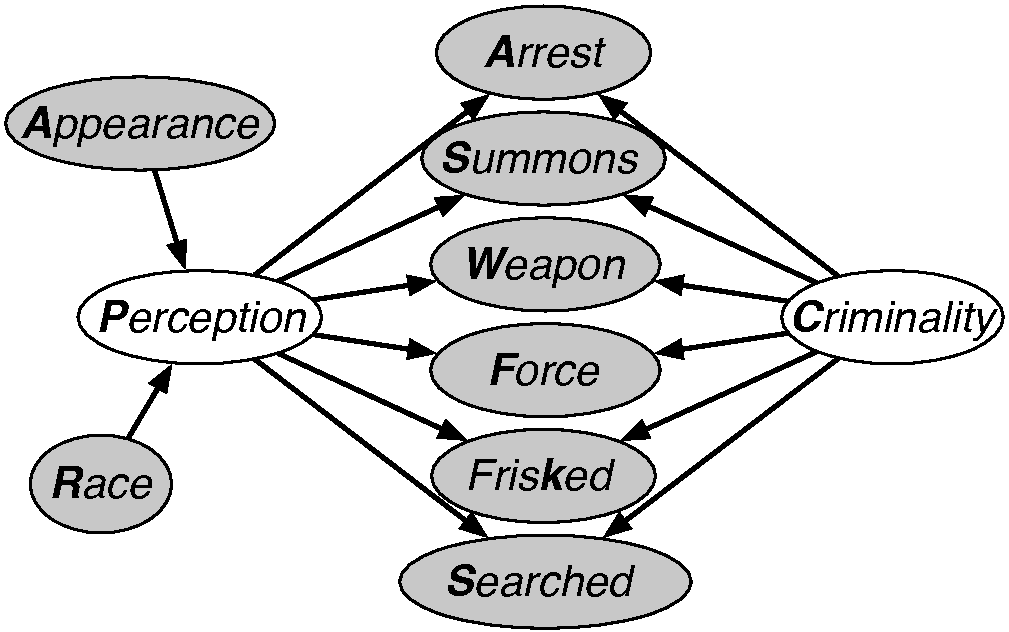
\includegraphics[width=\columnwidth]{stop_and_frisk_model3.pdf}}
\vspace{-2ex}
\caption{A causal model for the stop and frisk dataset.\label{figure.stop_and_frisk}\vspace{-4ex}}
\vspace{-2ex}
\end{center}
\end{figure}

\paragraph{Counterfactual fairness.}
We would like to empirically test whether the baseline methods are counterfactually fair. To do so we will assume the true model of the world is given by Figure~\ref{figure.law_school}, (\textbf{Level 2}). We can fit the parameters of this model using the observed data and evaluate counterfactual fairness by sampling from it. Specifically, we will generate samples from the model given either the observed race and sex, or \emph{counterfactual} race and sex variables. We will fit models to both the original and counterfactual sampled data and plot how the distribution of predicted FYA changes for both baseline models. Figure~\ref{figure.counterfactual} shows this, where each row corresponds to a baseline predictor and each column corresponds to the couterfactual change. In each plot, the blue distribution is density of predicted FYA for the original data and the red distribution is this density for the counterfactual data. If a model is counterfactually fair we would expect these distributions to lie exactly on top of each other. Instead, we note that the \textbf{Full} model exhibits counterfactual unfairness for all counterfactuals except sex. We see a similar trend for the \textbf{Unaware} model, although it is closer to being counterfactually fair. To see why these models seem to be fair w.r.t. to sex we can look at weights of the DAG which generates the counterfactual data. Specifically the DAG weights from (male,female) to GPA are ($0.93$,$1.06$) and from (male,female) to LSAT are ($1.1$,$1.1$). Thus, these models are fair w.r.t. to sex simply
because of a very weak causal link between sex and GPA/LSAT.

% here describe what we see

% maybe sample from model and check it out
%\paragraph{Model validity.}
 

% TODO rank top 10 students by ability or by other score in law_school.py which only considers observed features





% \begin{table}[t]
% \vspace{-2ex}
% \caption{}
% \vspace{-3ex}
% \label{table.pred_law}
% \begin{center}
% \resizebox{\columnwidth}{!}
% {
% \begin{sc}
% \footnotesize
% \begin{tabular}{c|c|c|c}
% \hline
% %\multicolumn{5}{c}{\textbf{Lower Bounds}}\\
% \hline
% & full & unaware  & fair l2 & fair l3 \\
% \hline
% RMSE & 0.873 & 0.894 & 0.929 & 0.918 \\ \hline
% \end{tabular}
% \end{sc}
% }
% \end{center}
% \vspace{-4ex}
% \end{table}

%{lr@{$\pm$}lr@{$\pm$}lr@{$\pm$}l}



\subsection{True vs. Perceived Criminality}
\label{sec:true-vs.-perceived}
Since 2002, the New York Police Department (NYPD) has recorded
information about every time a police officer has stopped someone. The
officer records information such as if the person was searched or
frisked, % if a weapon was found,
their appearance, % if force was used,
etc. We
consider the data collected on males stopped during 2014 which constitutes 38,609 records. % We limit our analysis to looking at just males stopped as this accounts for more than $90\%$ of the data.

\paragraph{Model.}
We model this stop-and-frisk data using the graph in Figure~\ref{figure.stop_and_frisk}. Specifically, we posit main causes for the observations: \emph{Arrest} (if an individual was arrested), \emph{Summons} (an individual was called to a court-summons), \emph{Weapon} (an individual was found to be carrying a weapon), \emph{Force} (some sort of force was used during the stop), \emph{Frisked}, and \emph{Searched}. The first cause of these observations is some measure of an individual's latent \emph{Criminality}, which we do not observe. We believe there is an additional cause, an individual's perceived criminality, \emph{Perception}, also unobserved. This second factor is introduced as we believe that these observations may be biased based on an officer's perception of whether an individual is likely a criminal or not. This perception is affected by an individual's \emph{Appearance} and their \emph{Race}. In this sense \emph{Criminality} is counterfactually fair, while \emph{Perception} models how race affects each of the other observed variables.

\paragraph{Criminality and perception distributions.}
After fitting this model to the data we can look at the distribution of \emph{Criminality} and \emph{Perception} across different races, shown as box plots in Figure~\ref{figure.stop_and_frisk}. We see that the median criminality for each race is nearly identical, while the distributions are somewhat different, demonstrating that \emph{Criminality} approaches demographic parity. The differences that due exist may be due to unobserved confounding variables that are affected by race or unmodeled noise in the data. On the right \emph{Perception} varies considerably by race with white individuals having the lowest perceived criminality while black and black Hispanic individuals have the highest.

\begin{figure}[!th]
\begin{center}
%\vspace{-1ex}
\centerline{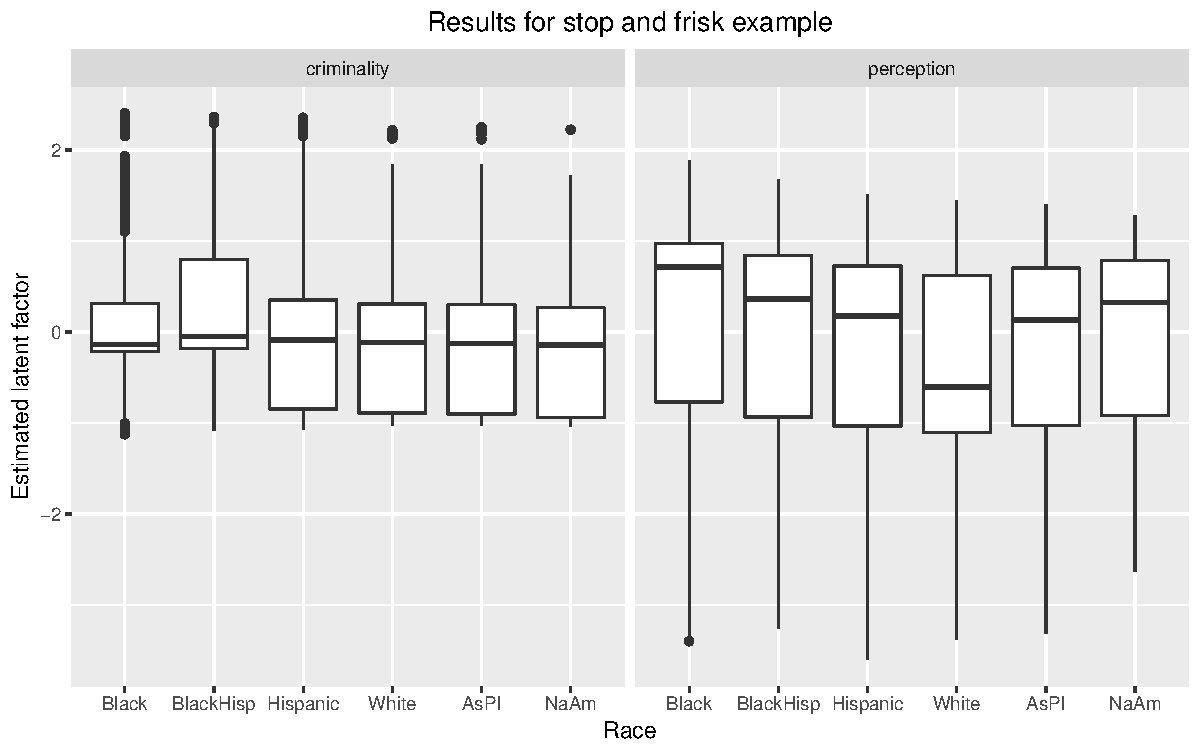
\includegraphics[width=\columnwidth]{stopandfrisk_output.pdf}}
\vspace{-2ex}
\caption{Distributions of estimated latent perception and criminality scores for the stop and frisk dataset.\label{figure.stop_and_frisk_output}\vspace{-5ex}}
\vspace{-2ex}
\end{center}
\end{figure}

\paragraph{Visualization on a map of New York City.}
Each of the stops can be mapped to longitude and latitude points for where the stop occurred\footnote{https://github.com/stablemarkets/StopAndFrisk}. Thus we can visualize \emph{Criminality} and \emph{Perception} alongside \emph{Race} and the combination of \emph{Arrest} and \emph{Summons}, shown in Figure~\ref{figure.criminality}.  Criminality seems to be a continuous approximation of arrest and summons as both plots show red in similar areas. However, the plots show that certain areas, while having a lot of arrests have low criminality scores such as south Bronx and west Queens (circled in orange). We can also compare the perceived criminality with a plot of race, where we have divided the races into Group A: black, black Hispanic, Hispanic, and Native American (shown in purple); and Group B: white and Asian/Pacific Islander (shown in green). Group A are all races that have positive weights on the connection from \emph{Race} to \emph{Perception} in the fitted model, while Group B all have negative weights. Thus being in Group A leads one to have a higher perceived criminality than being in Group B. This can be seen in the right-most plot of Figure~\ref{figure.criminality}. Certain areas of town such as central Brooklyn, central Bronx, and southern Queens have very high criminality and almost all stops are by members of Group A (circled in yellow).




%\subsection{Model criticism}
%%% Local Variables:
%%% mode: latex
%%% TeX-master: "ricardo_draft"
%%% End:
